\section{Kelayakan}
\label{sec:kelayakan}

\subsection{Hasil Simulasi: Paket Seimbang}

Eksplorasi kombinasi kebijakan menemukan satu paket yang membuat neraca PLN tidak lagi negatif (H3). Paket seimbang memensiunkan empat PLTU IPP tua pada 2030, yaitu Cirebon-1, Tanjung Jati B unit 1-2, dan Cilacap unit 1-2 dengan total 2.580 MW. Paket ini juga memasang 100 MW per tahun PLTS atap di gedung pemerintah tanpa mengubah nilai ekspor, dengan 75\% kompensasi dari dana luar. Hasilnya, neraca PLN $+$Rp1,4 triliun, neraca negara $+$Rp3,5 triliun, dana luar Rp14,7 triliun, dan sekitar 8.900 kematian dini dihindari atau setara Rp103,7 triliun (Tabel~\ref{tab:preset}).

\begin{figure}[H]
\centering
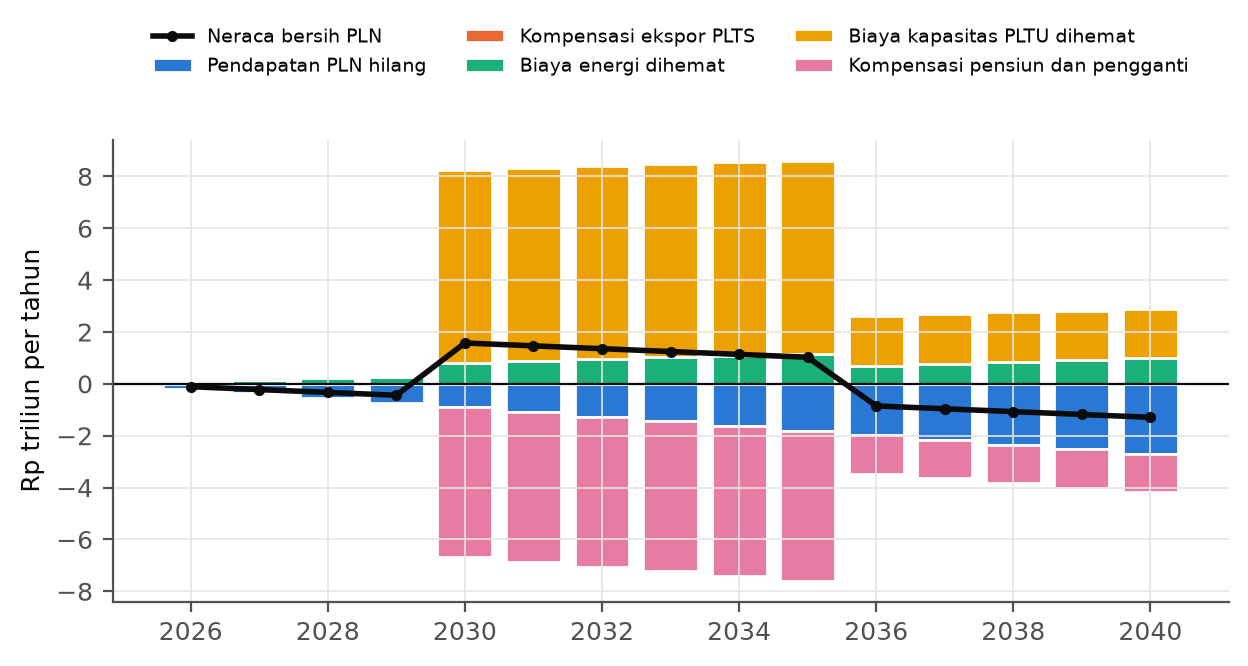
\includegraphics[width=\textwidth]{neraca_seimbang}
\caption{Komponen neraca PLN per tahun pada Paket seimbang}
\label{fig:seimbang}
\sumber{simulasi PowerShift}
\end{figure}

Gambar~\ref{fig:seimbang} menjelaskan sumber keseimbangan itu. Selama 2030-2035, PLN menghemat pembayaran kapasitas IPP sekitar Rp7 triliun per tahun. Penghematan ini mengimbangi porsi kompensasi dan biaya 2.580 MW pembangkit pengganti. Setelah 2036, tiga dari empat PLTU memang sudah pensiun di baseline, sehingga selisihnya mengecil. Gambar~\ref{fig:rm} menunjukkan bahwa tanpa pembangkit pengganti, reserve margin akan turun ke 25,9\%. Karena itu, biaya pengganti dihitung sebagai bagian dari paket.

\begin{figure}[H]
\centering
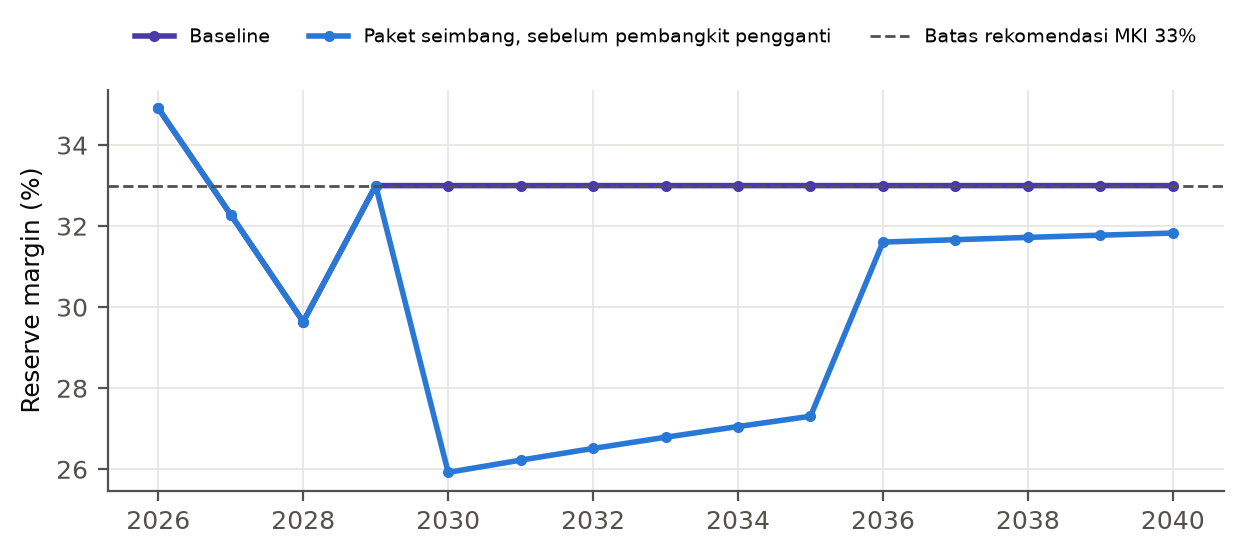
\includegraphics[width=\textwidth]{reserve_margin}
\caption{Reserve margin baseline dan Paket seimbang sebelum pembangkit pengganti}
\label{fig:rm}
\sumber{simulasi PowerShift berdasarkan \textcite{B-MATAHARI-2024} dan \textcite{B-PETROMINDO-RESERVE}}
\end{figure}

Pilihan PLTU sangat menentukan. Pensiun PLTU milik PLN, misalnya Pelabuhan Ratu, justru membebani PLN karena tidak ada pembayaran kapasitas yang dapat dihemat, sementara nilai buku dan pembangkit pengganti tetap harus ditanggung. Sebaliknya, Cirebon-1 memberi manfaat kesehatan terbesar per MW karena lokasinya.

\subsection{Biaya dan Pelaksana}

Biaya pengembangan PowerShift hanya waktu kerja tim. Biaya operasinya nol karena berupa situs statis dengan hosting gratis dan data terbuka. Pelaksana yang diusulkan:
\begin{itemize}
  \item \textbf{Ditjen Ketenagalistrikan ESDM dan tim kerja gabungan Pasal 14 Permen ESDM 10/2025}: pengguna utama untuk menilai usulan pensiun dini.
  \item \textbf{PLN}: mengganti parameter kontrak IPP dengan data sebenarnya saat menyusun kajian enam bulan.
  \item \textbf{Dinas ESDM Jawa Barat}: menyorot Cirebon-1 dan kontribusi PLTS atap provinsi.
  \item \textbf{Kampus atau lembaga riset energi}: memelihara data dan model sebagai barang publik.
\end{itemize}

\subsection{Kebijakan Pendukung}

PowerShift memanfaatkan kerangka yang sudah ada. Permen ESDM 10/2025 mewajibkan kajian teknis, hukum, komersial, dan keuangan serta membuka penggunaan kajian lembaga independen sebagai rujukan \parencite{B-CNN-20250422}. Kuota PLTS atap 5.746 MW untuk 2024-2028 \parencite{B-PVMAG-QUOTA} dan rencana 33,5 GW pembangkit baru di Jamali, termasuk 10,9 GW surya \parencite{B-LISTRIKID-RUPTL-JAMALI}, memberi ruang untuk menguji paket. Usulan IESR untuk mengalihkan subsidi 450/900 VA ke PLTS atap \parencite{B-KABARBURSA-SUBSIDI} juga dapat diuji langsung di alat.

\subsection{Risiko}

\begin{figure}[H]
\centering
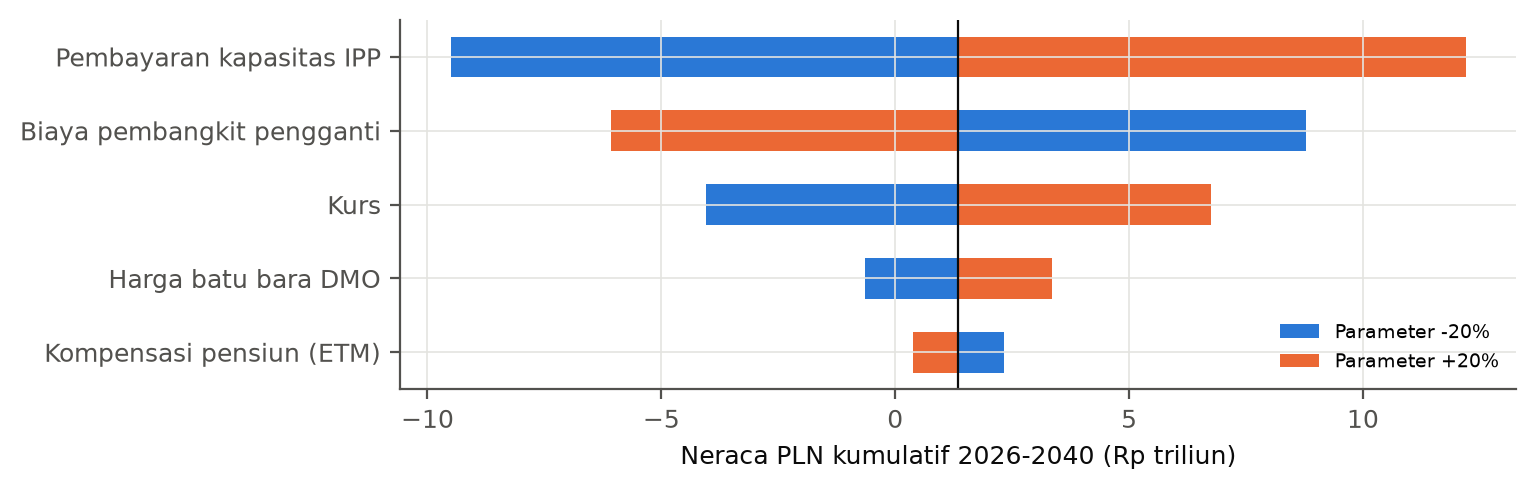
\includegraphics[width=\textwidth]{tornado_seimbang}
\caption{Sensitivitas neraca PLN Paket seimbang terhadap perubahan parameter $\pm$20\%}
\label{fig:tornado}
\sumber{simulasi PowerShift}
\end{figure}

Risiko terbesar adalah ketidakpastian data kontrak IPP. Gambar~\ref{fig:tornado} menunjukkan bahwa neraca Paket seimbang paling peka terhadap besaran pembayaran kapasitas IPP dan biaya pembangkit pengganti. Perubahan 20\% dapat menggeser hasil sekitar Rp7-11 triliun. Risiko lain adalah klaim kompensasi yang jauh lebih tinggi. Dengan klaim PLN untuk Cirebon-1 (sekitar Rp18 miliar per MW per tahun dipercepat), neraca PLN memburuk tajam. Mitigasinya, semua asumsi ditampilkan terbuka dan dapat diubah, sehingga perbedaan angka antara PLN, ADB, dan pemerintah dapat diperdebatkan secara transparan. Model ini juga tidak menggantikan simulasi jaringan per jam, sehingga hasilnya bersifat indikatif.

\subsection{Ukuran Keberhasilan}

\begin{itemize}
  \item Teknis: halaman terbuka di bawah 3 detik, perhitungan ulang instan, hitung tangan cocok dengan aplikasi (sudah tercapai).
  \item Isi: minimal 70\% parameter kunci berstatus terverifikasi. Saat ini 18 dari 42 parameter terverifikasi, 21 asumsi terdokumentasi, dan 3 masih perlu dicek ke sumber asli.
  \item Pemakaian: PowerShift dipakai dalam minimal satu diskusi kebijakan atau kajian pensiun dini, dan skenario dibagikan antarpemangku kepentingan.
\end{itemize}
